\section{Hardware Structure}

\begin{figure}[h] % h means put this image here
	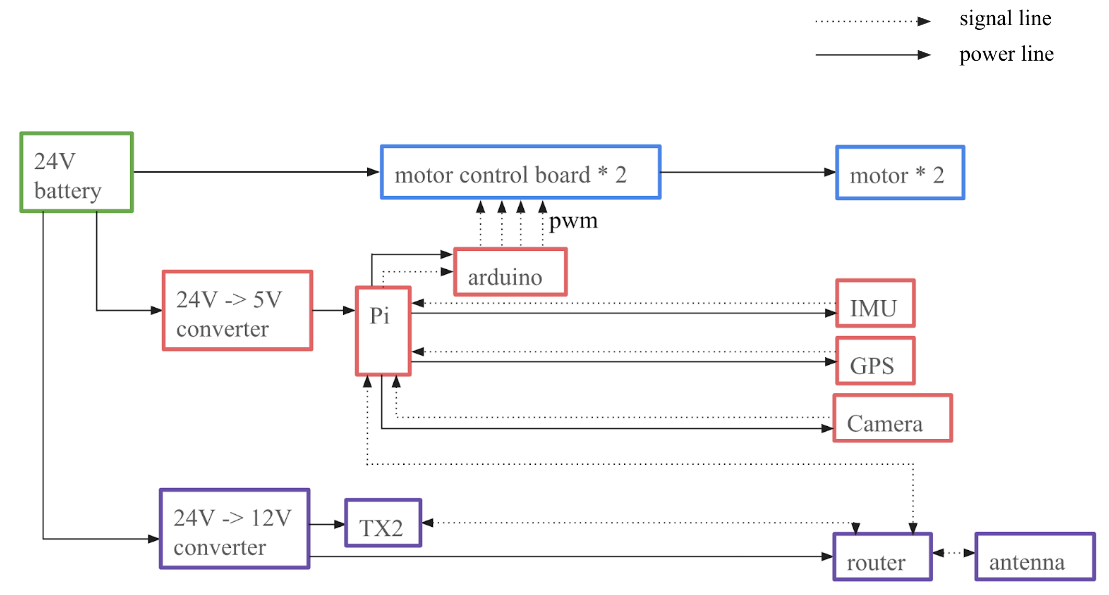
\includegraphics[width=0.8\columnwidth]{images/hardware.png}
	\centering
	\caption{signal and power flow}
	\label{figure:hardware}
\end{figure}

\subsection{Power Transmition}

For power transmission, this system needs 3 kinds of voltages, 24V, 5V, and 12V. 24V supply through two motor control boards then drive the two motors. 5V supply initially powered Raspberry pi, it will also supply Arduino UNO, IMU, GPS and pi camera with it’s USB ports. As to 12V, it will supply TX2 compute unit and router.

\subsection{Signal Transmition}

For signal transmission, Raspberry pi and TX2 will communicate through wifi, wifi router with an antenna will set on the boat. The Raspberry pi will collect the data from IMU, GPS and pi camera, after computing in Raspberry pi and image processing in TX2, it will send pwm signal (0~3.3V) to Arduino UNO, then Arduino will map the input signal from (0~3.3V) into (0~5V) to two motor control boards.

\subsection{hardware setting}
Most of the compute units and sensors mentioned above except two motors, GPS and antenna, will be placed in a waterproof box. There will have waterproof connectors while the wire needs to go out from the waterproof box.

\begin{figure}[h] % h means put this image here
	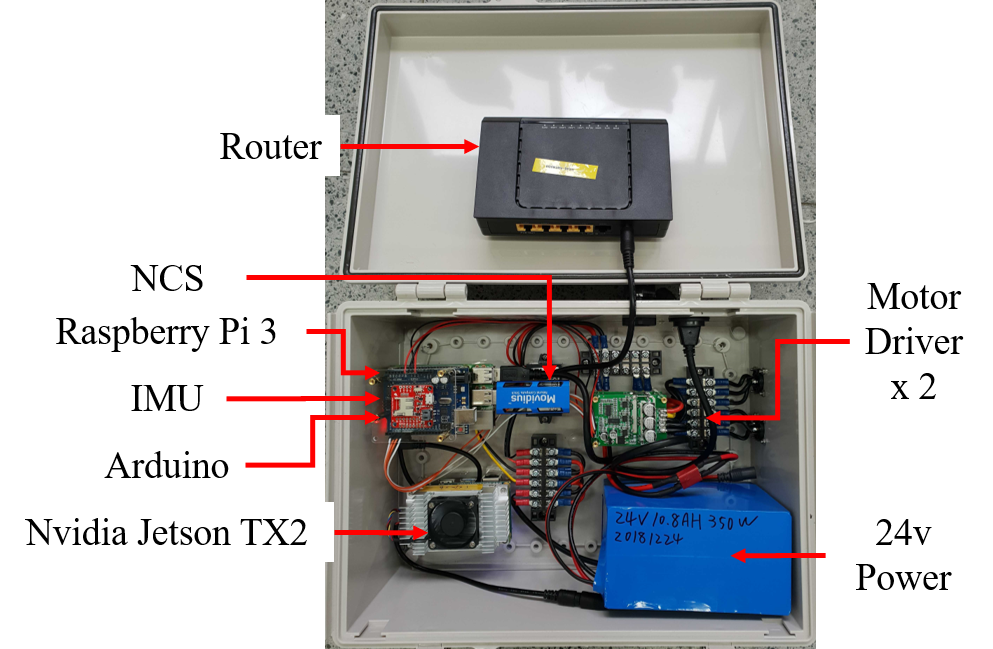
\includegraphics[width=0.8\columnwidth]{images/hardware_setting.png}
	\centering
	\caption{hardware setting}
	\label{figure:hardware_setting}
\end{figure}

\begin{figure}[h] % h means put this image here
	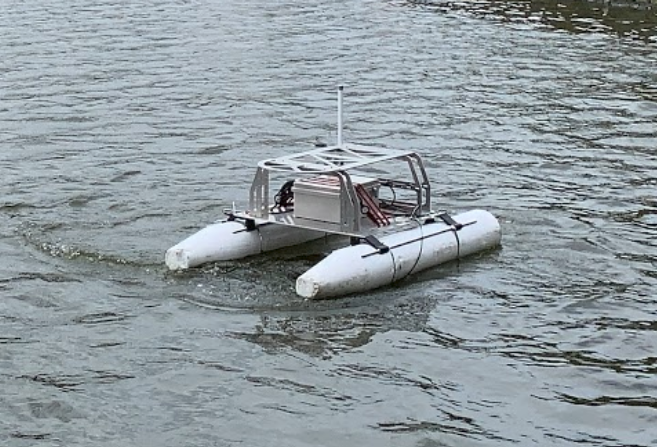
\includegraphics[width=0.8\columnwidth]{images/duckieboat.png}
	\centering
	\caption{The appearance of Duckieboat and where the waterproof box was placed.}
	\label{figure:duckieboat}
\end{figure}
